\section{How straight are the crests}\label{sec:results}

How does the straightness of the crests depend on the scale, and do the Alps and the Pyrenees differ? The crests are the
paths of the construction of Section~\ref{sec:crestpaths}, measured by the TAMSD of a ball that runs along them at constant
speed (Section~\ref{sec:tamsd}). Figure~\ref{fig:tamsd} shows the answer as a function of the arc length $s$, and
Table~\ref{tab:hgeo} gives the exponent on windows of $s$.

\begin{figure}
\centering
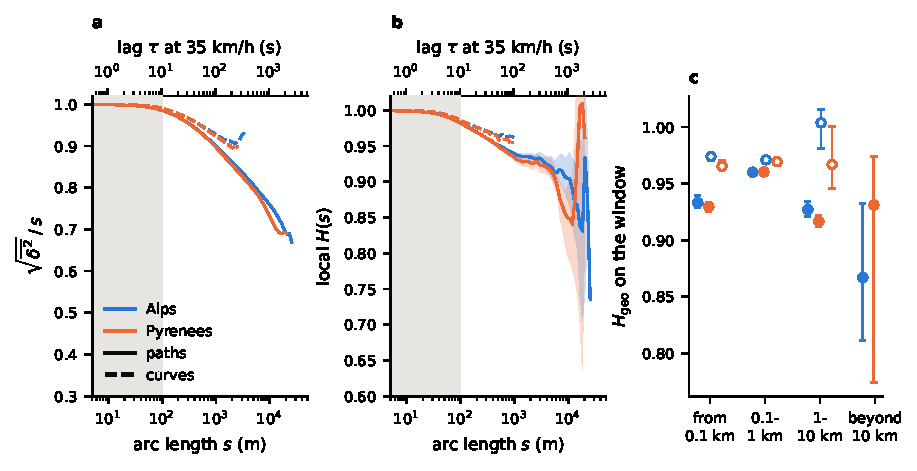
\includegraphics[width=\textwidth]{figures/tamsd.pdf}
\caption{The crests bend more at larger scales, in the Alps and the Pyrenees alike. Alps in indigo, Pyrenees in olive; paths solid,
single curves dashed. \textbf{a}~End-to-end distance over arc length, $\sqrt{\overline{\delta^2}}/s$, which is 1 on a straight
line. Bottom axis: arc length $s$; top axis: lag $\tau$ of a ball at 35~km/h; grey: below four cells, where the grid sets the
shape. \textbf{b}~Local slope of the MSD, $\alpha(s)$, Eq.~\eqref{eq:alphaloc}, with the 95\% band for the paths. Dashed horizontal
lines: $\Hgeo$ of the window from 0.1~km (Table~\ref{tab:hgeo}), over the lags of that fit. Curves are drawn where at least 100
paths reach the lag and the band is narrower than 0.05.}
\label{fig:tamsd}
\end{figure}

\begin{table}[H]
\centering
\caption{$\Hgeo$ on windows of arc length $s$, with 95\% bootstrap intervals (over trees for the paths, over curves for the
curves). The Alps and the Pyrenees agree between 0.1 and 1~km. Single curves are too short for the last window.}
\label{tab:hgeo}
\small
\setlength{\tabcolsep}{4pt}
\begin{tabular}{lllll}
\toprule
 & \multicolumn{2}{c}{Alps} & \multicolumn{2}{c}{Pyrenees} \\
\cmidrule(lr){2-3}\cmidrule(lr){4-5}
window of $s$ & paths & curves & paths & curves \\
\midrule
from 0.1~km & 0.933 (0.929--0.940) & 0.974 (0.970--0.977) & 0.930 (0.925--0.933) & 0.965 (0.962--0.970) \\
0.1--1~km & 0.960 (0.959--0.961) & 0.971 (0.971--0.972) & 0.960 (0.959--0.962) & 0.969 (0.969--0.970) \\
1--10~km & 0.927 (0.921--0.934) & 1.004 (0.981--1.015) & 0.917 (0.912--0.922) & 0.967 (0.946--1.000) \\
beyond 10~km & 0.867 (0.812--0.933) & -- & 0.931 (0.774--0.974) & --
\\
\bottomrule
\end{tabular}
\end{table}

The local slope falls with the scale and has no plateau. In the Alps it goes from \CgAlpsPathsAlphaHundred{} at 100~m to
\CgAlpsPathsAlphaFiveKm{} at 5~km, and the Pyrenees give the same picture. The exponent therefore depends on the window it is
fitted on, and the flights are compared with the function $\alpha(s)$ as well as with one number.

From 0.1~km on, $\Hgeo$ of the paths is \CgAlpsPathsFrom{} in the Alps and \CgPyrPathsFrom{} in the Pyrenees, with
overlapping intervals. The two massifs agree between 0.1 and 1~km; between 1 and 10~km the Pyrenees are slightly lower; beyond
10~km the intervals are wide, since the window rests on few trees.

Single curves are straighter than the paths. The value of the curves over 1 to 10~km mixes populations, because only the
longest curves reach the large lags, so the paths are used for every comparison.

Three things limit the exponent: the edge of the elevation data, the grid scale and the number of trees at long lags. It holds
from 100~m to a few kilometres; beyond 10~km it is an estimate with a wide interval. Appendix~\ref{app:limits} shows each limit.

\paragraph{What we keep.} The crests are close to straight from 100~m up and bend more as the scale grows, so no single
exponent describes them. The Alps and the Pyrenees agree up to 1~km and differ little beyond.
